%package list
\documentclass{article}
\usepackage[top=3cm, bottom=3cm, outer=3cm, inner=3cm]{geometry}
\usepackage{graphicx}
\usepackage{url}
%\usepackage{cite}
\usepackage{hyperref}
\usepackage{array}
%\usepackage{multicol}
\newcolumntype{x}[1]{>{\centering\arraybackslash\hspace{0pt}}p{#1}}
\usepackage{natbib}
\usepackage{pdfpages}
\usepackage{multirow}
\usepackage{multirow}
\usepackage[T1]{fontenc}
\usepackage{imakeidx}
% Imagenes de costado
\usepackage{wrapfig}
\usepackage{graphicx}

% Modificar URLs
\usepackage{hyperref}
\hypersetup{
    colorlinks=true,
    linkcolor=black,
    filecolor=magenta,      
    urlcolor=blue,
    pdftitle={Overleaf Example},
    pdfpagemode=FullScreen,
    }

\urlstyle{same}


\usepackage[normalem]{ulem}
\useunder{\uline}{\ul}{}

\usepackage{minted}

% codigo fuente
\usepackage{listings}
\usepackage{color, colortbl}
\definecolor{dkgreen}{rgb}{0,0.6,0}
\definecolor{gray}{rgb}{0.5,0.5,0.5}
\definecolor{mauve}{rgb}{0.58,0,0.82}
\definecolor{codebackground}{rgb}{0.95, 0.95, 0.92}
\definecolor{tablebackground}{rgb}{0.0, 0.45, 0.63}
\lstset{frame=tb,
	language=bash,
	aboveskip=3mm,
	belowskip=3mm,
	showstringspaces=false,
	columns=flexible,
	basicstyle={\small\ttfamily},
	numbers=none,
	numberstyle=\tiny\color{gray},
	keywordstyle=\color{blue},
	commentstyle=\color{dkgreen},
	stringstyle=\color{mauve},
	breaklines=true,
	breakatwhitespace=true,
	tabsize=3,
	backgroundcolor= \color{codebackground},
}

%%%%%%%%%%%%%%%%%%%%%%%%%%%%%%%%%%%%%%%%%%%%%%%%%%%%%%%%%%%%%%%%%%%%%%%%%%%%
%%%%%%%%%%%%%%%%%%%%%%%%%%%%%%%%%%%%%%%%%%%%%%%%%%%%%%%%%%%%%%%%%%%%%%%%%%%%
\newcommand{\csemail}{vmachacaa@ulasalle.edu.pe}
\newcommand{\csdocente}{MSc. Maribel Molina Barriga}
\newcommand{\cscurso}{Sistemas Operativos}
\newcommand{\csuniversidad}{Universidad La Salle}
\newcommand{\csescuela}{Escuela Profesional de Ingeniería de Software}
\newcommand{\cspracnr}{03}
\newcommand{\cstema}{Instalación Distros}
%%%%%%%%%%%%%%%%%%%%%%%%%%%%%%%%%%%%%%%%%%%%%%%%%%%%%%%%%%%%%%%%%%%%%%%%%%%%
%%%%%%%%%%%%%%%%%%%%%%%%%%%%%%%%%%%%%%%%%%%%%%%%%%%%%%%%%%%%%%%%%%%%%%%%%%%%


\usepackage[english,spanish]{babel}
\usepackage[utf8]{inputenc}
\AtBeginDocument{\selectlanguage{spanish}}
\renewcommand{\figurename}{Figura}
\renewcommand{\refname}{Referencias}
\renewcommand{\tablename}{Tabla} %esto no funciona cuando se usa babel
\AtBeginDocument{%
	\renewcommand\tablename{Tabla}
}

\usepackage{fancyhdr}
\pagestyle{fancy}
\fancyhf{}
\setlength{\headheight}{30pt}
\renewcommand{\headrulewidth}{1pt}
\renewcommand{\footrulewidth}{1pt}
\fancyhead[L]{\raisebox{-0.2\height}{
\includegraphics[width=3cm]{logo_ulasalle (1).png}}}
\fancyhead[C]{}
\fancyhead[R]{\fontsize{7}{7}\selectfont	\csuniversidad \\ \csescuela \\ \textbf{\cscurso} }
\fancyfoot[L]{}
\fancyfoot[C]{Sistemas Operativos}
\fancyfoot[R]{Página \thepage}



\begin{document}

	\vspace*{10px}
	
	\begin{center}	
		\fontsize{17}{17} \textbf{ Práctica \cspracnr}
	\end{center}
	%\centerline{\textbf{\underline{\Large Título: Informe de revisión del estado del arte}}}
	%\vspace*{0.5cm}
	

\renewcommand{\arraystretch}{1.5}
\begin{table}[h]
	\begin{tabular}{|x{4.7cm}|x{4.8cm}|x{4.8cm}|}
		\hline 
		\textbf{DOCENTE} & \textbf{CARRERA}  & \textbf{CURSO}   \\
		\hline 
		\csdocente & \csescuela & \cscurso    \\
		\hline 
	\end{tabular}
\end{table}	

\begin{table}[h]
	\begin{tabular}{|x{4.7cm}|x{4.8cm}|x{4.8cm}|}
		\hline 
		\textbf{GRUPO} & \textbf{TEMA}  & \textbf{DURACIÓN}   \\
		\hline 
		\ 6 & \cstema & 5 horas   \\
		\hline 
	\end{tabular}
\end{table}
\renewcommand{\arraystretch}{1} 
	\section*{Integrantes}
	 	\begin{itemize}
                    \item José Carlos Machaca Vera
	 		\item Jhosep Alonso Mollapaza Morocco
	 		\item Patrick Andres Ramirez Santos
	 \end{itemize}
 
	\tableofcontents


	

\newpage

\section{Objetivos}
\begin{itemize}
    \item Instalar 2 distribuciones de Linux, en este caso Manjaro y UwUntu utilizando máquinas virtuales
    \item Crear y ejecutar programas en las distribuciones instaladas
    \item Crear una guía de instalacion eficiente y concisa
\end{itemize}

\section{Instalación Manjaro minimal}
    \subsection{VirtualBox}
    Manjaro no dispone de una version minima para arquitecturas x86, solamente para ARM y debido a la dificultad de virtualizar dicho entorno se procedio a instalar la version grafica minimal, para lo cual se configuró la máquina virtual de la siguiente forma:
        \\ 
        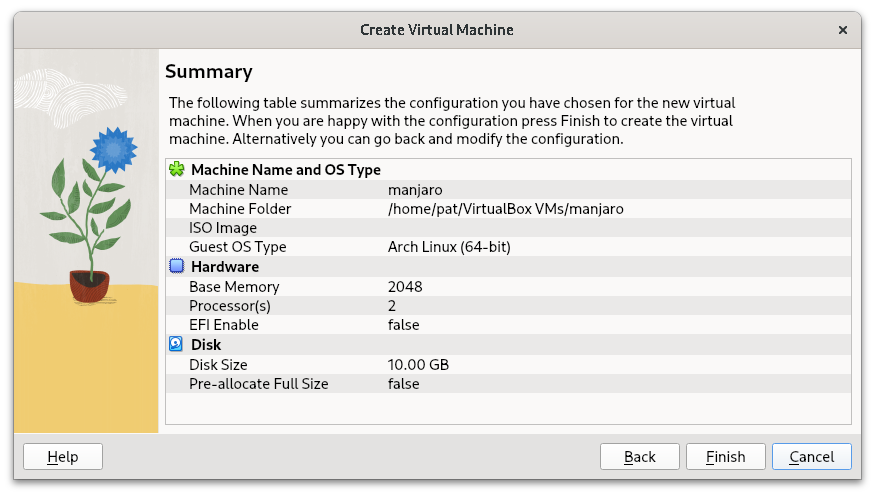
\includegraphics[scale=0.5]{vm/init.png}
        
\newpage
    \subsection{Instalacion}
    Se asignó 10 GB de almacenamiento, 2 GB de RAM y 2 procedores. Todo esto se realizó a lo largo de varias interfaces descritas así:
    \\
    \begin{tabular}{cc}
        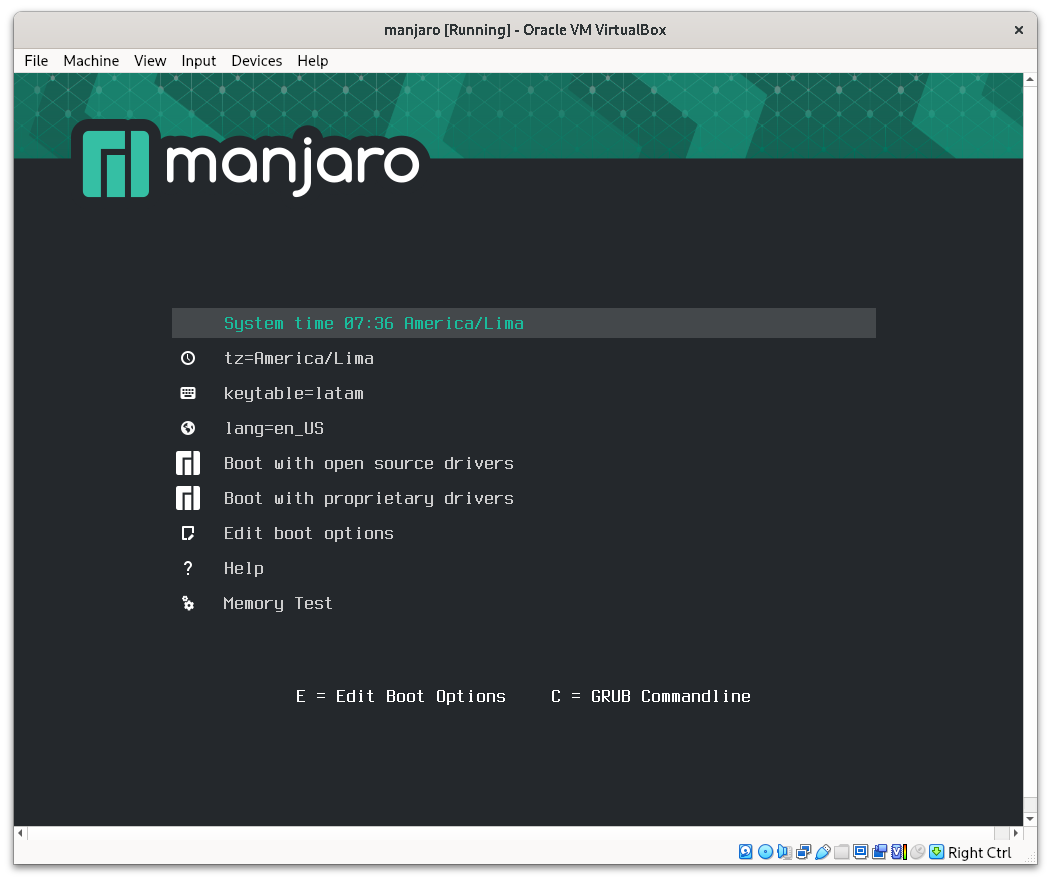
\includegraphics[width=.4\linewidth,valign=m]{vm/boot.png} & 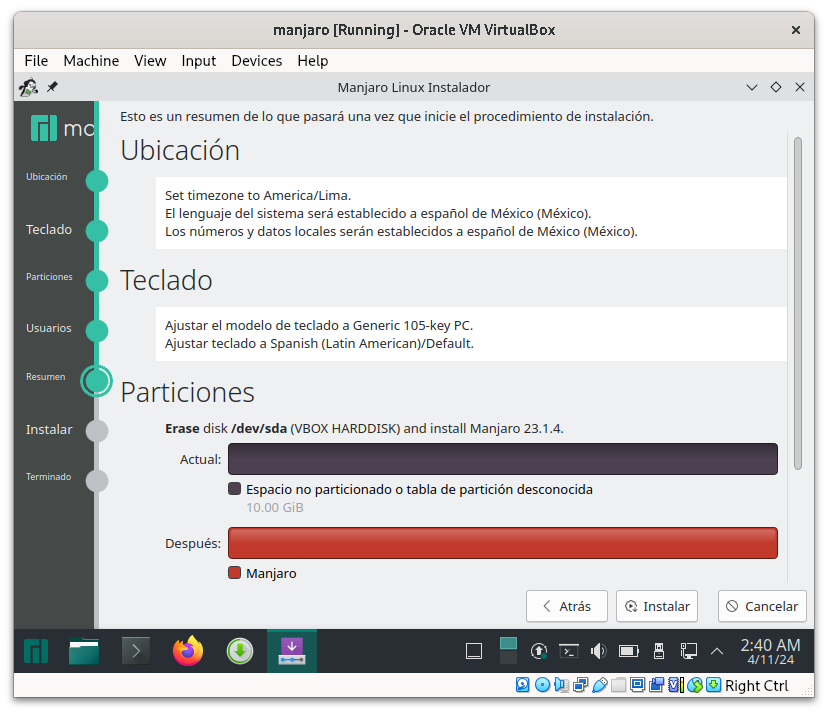
\includegraphics[width=.4\linewidth,valign=m]{vm/detalles.png} \\
        Boot & Resumen \\
        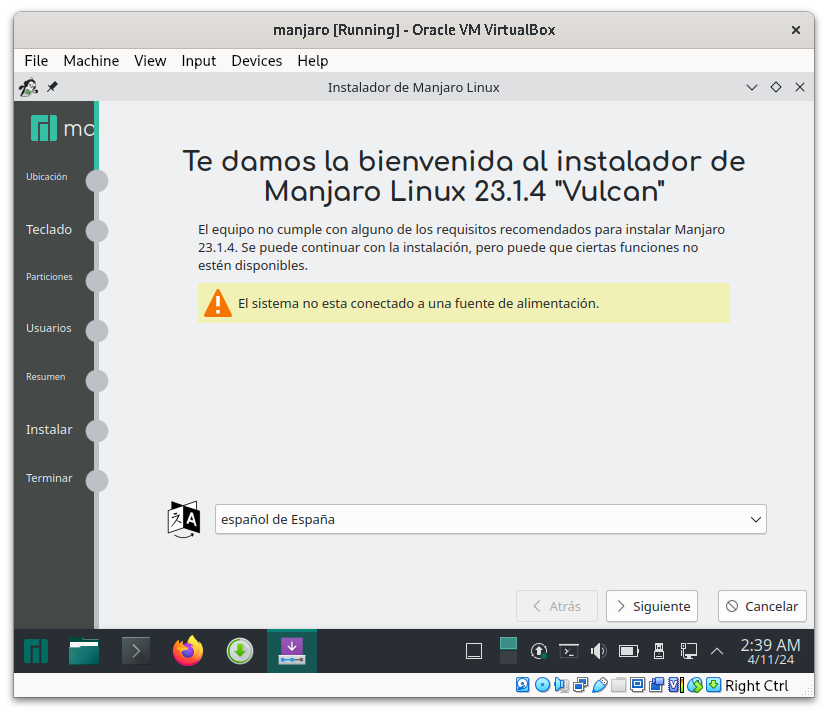
\includegraphics[width=.4\linewidth,valign=m]{vm/instalacion.png} & 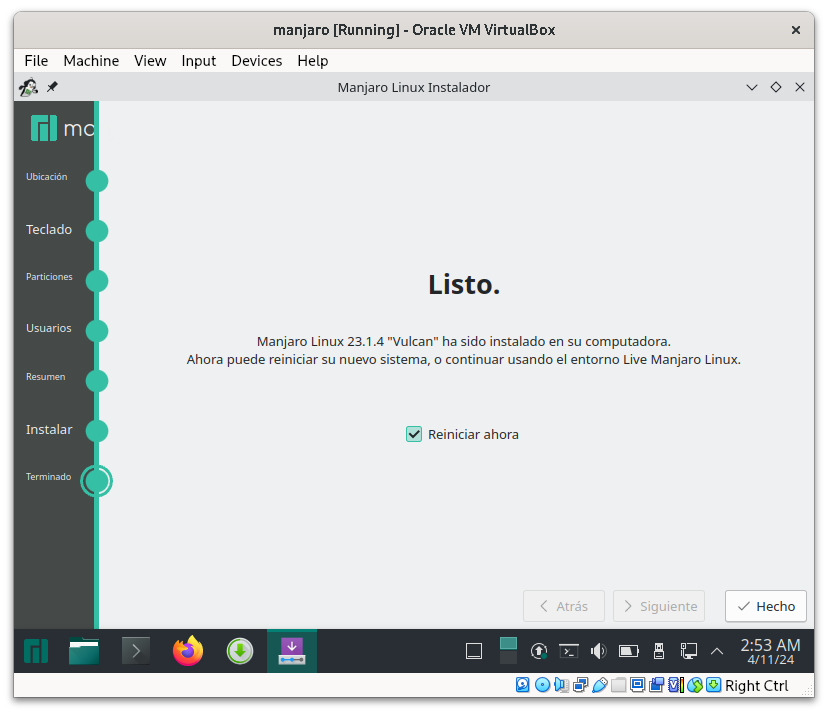
\includegraphics[width=.4\linewidth,valign=m]{vm/final.png} \\
        Menu inicial & Menu cierre \\
    \end{tabular}

\newpage
\section{Instalacion de paquetes}
Se instala los compiladores usando base-devel, se añade vim, tree y screenfetch. TOdo esto se realiza con los siguientes comandos y finalmente se muestra una imagen con los paquetes instalados usando la flag -Q de pamac:
    
    \begin{minted}[tabsize=2,breaklines]{bash}
        $ pamac install base-devel
        $ pamac install vim
        $ pamac install tree
        $ pamac install screenfetch
        $ pamac -Q [Nombe del paquete]
    \end{minted}

    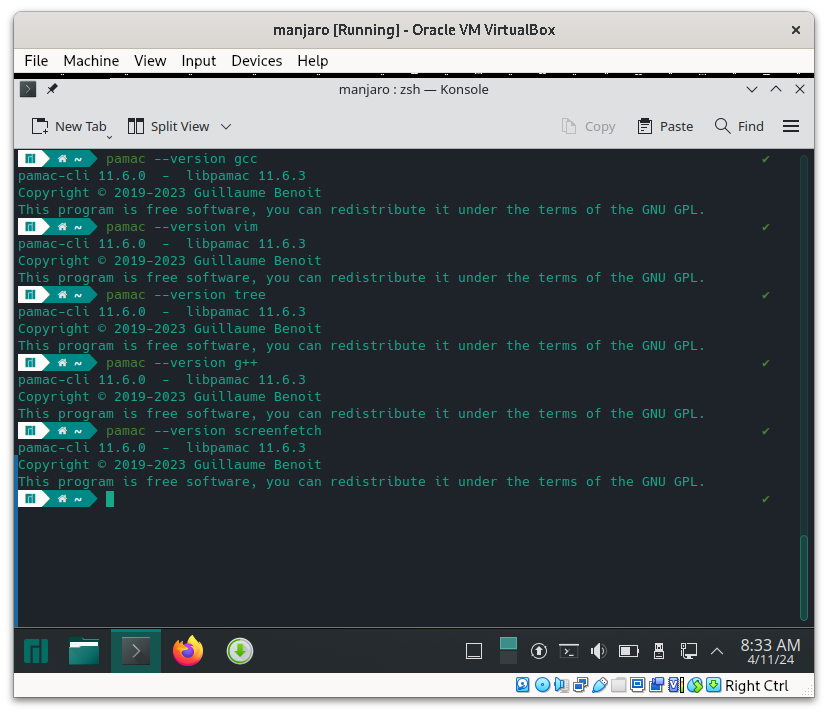
\includegraphics[scale=0.5]{vm/paquetes.png}
\newpage
Ademas se muestran los resultados de los comandos:
    \begin{minted}[tabsize=2,breaklines]{bash}
        $ uname -a
        $ screenfetch
    \end{minted}
    
    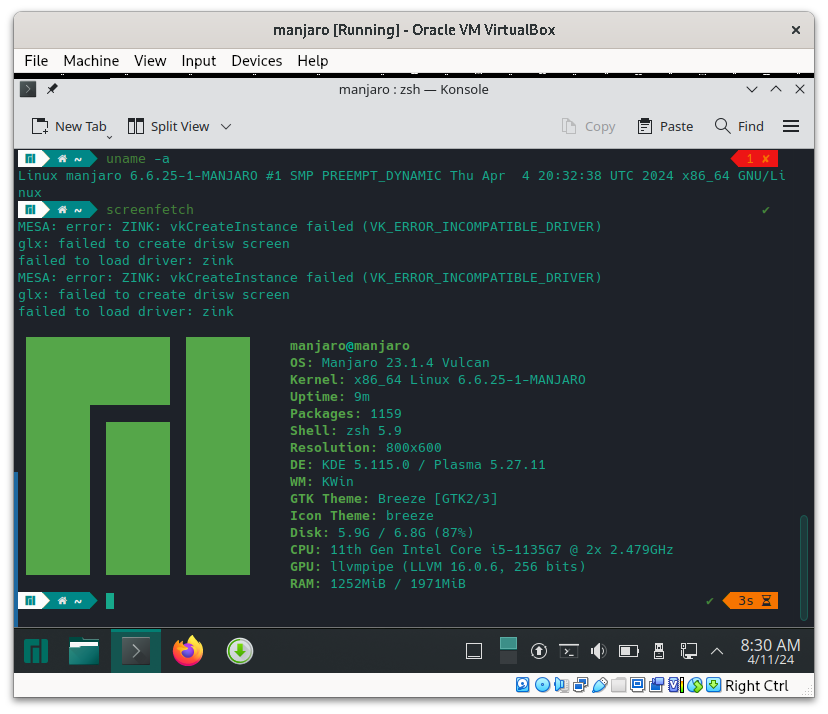
\includegraphics[scale=0.5]{vm/comandos.png}

\newpage

\section{Instalación UwUntu}

   \subsection{VirtualBox}
    UwUntu al ser una distro de Ubuntu y que usa Ubuntu Budgie 10.6.1 que es conocido por ser simple y elegante, diseñado para ser fácil de usar, entonces la instalación de UwUntu por medio de VirtualBox no ha sido un problema solo hay que tener espacio ya que cuenta con varios paquetes y programas preinstalados, porque esta pensado para usuarios dedicados a los videojuegos y a la cultura popular.

    Se configuro la máquina virtual de la siguiente forma.
        \\ 
    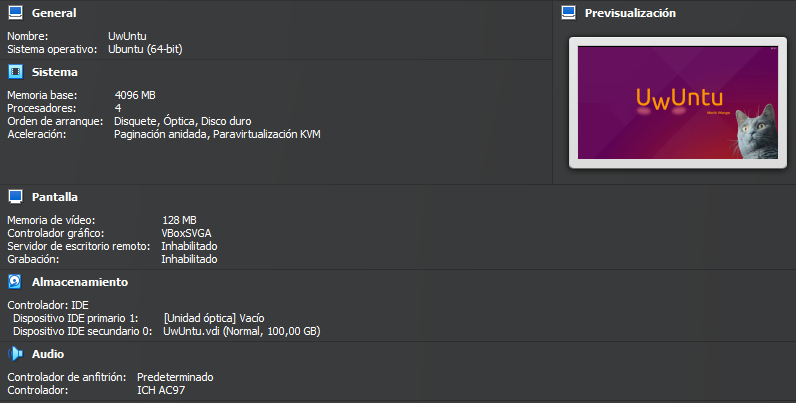
\includegraphics[scale=0.7]{Uwuntu/VirtualDescripcion.png}
\newpage
    \subsection{Instalacion}
    Para este sistema se asigno 100 GB de almacenamiento, 4 GB de RAM y 4 procesadores. Estas son los procesos de instalación que realiza UwUntu:
    \\
    \\
    \begin{tabular}{cc}
        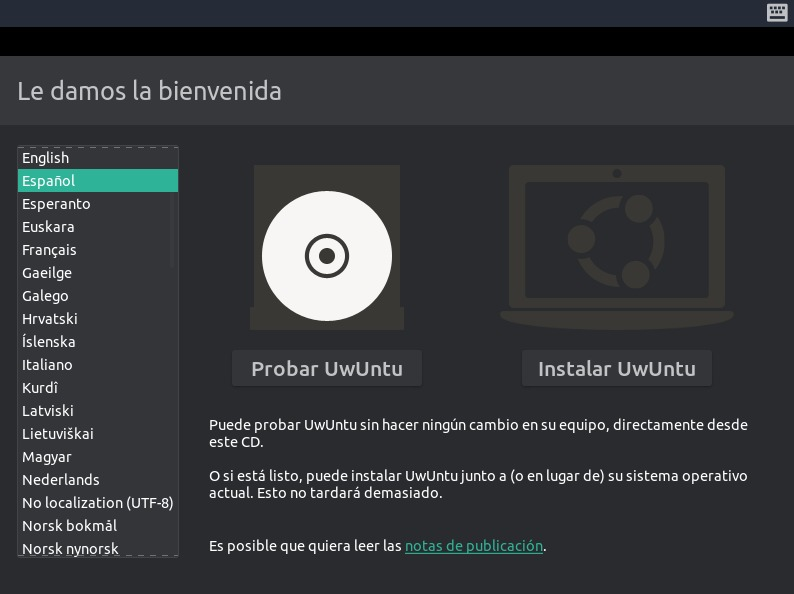
\includegraphics[width=.5\linewidth,valign=m]{Uwuntu/Menu inicial.png} & \includegraphics[width=.5\linewidth,valign=m]{Uwuntu/Instalación.png} \\
        Menu Inicial & Instalación \\
        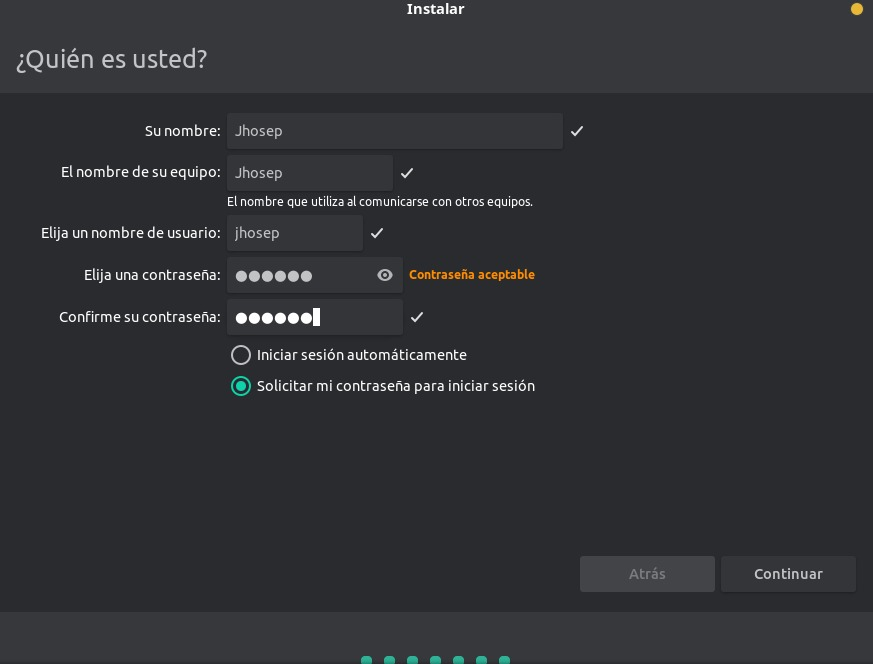
\includegraphics[width=.5\linewidth,valign=m]{Uwuntu/Usuario.png} & 
\includegraphics[width=.5\linewidth,valign=m]{Uwuntu/Escritorio.png} \\
        Usuario & Escritorio \\
    \end{tabular}
\newpage
    \section{Instalacion de paquetes}
Se instala los compiladores, vim, tree y screenfetch solicitados mediante la consola:
    
    \begin{minted}[tabsize=2,breaklines]{bash}
        UwU sudo apt install gcc
        UwU sudo apt install vim
        UwU sudo apt install tree
        UwU sudo apt install g++
        UwU sudo apt install screenfetch
    \end{minted}
    
    Y se muestran las versiones para demostrar que fueron instaladas.
    \\
    \\ 

    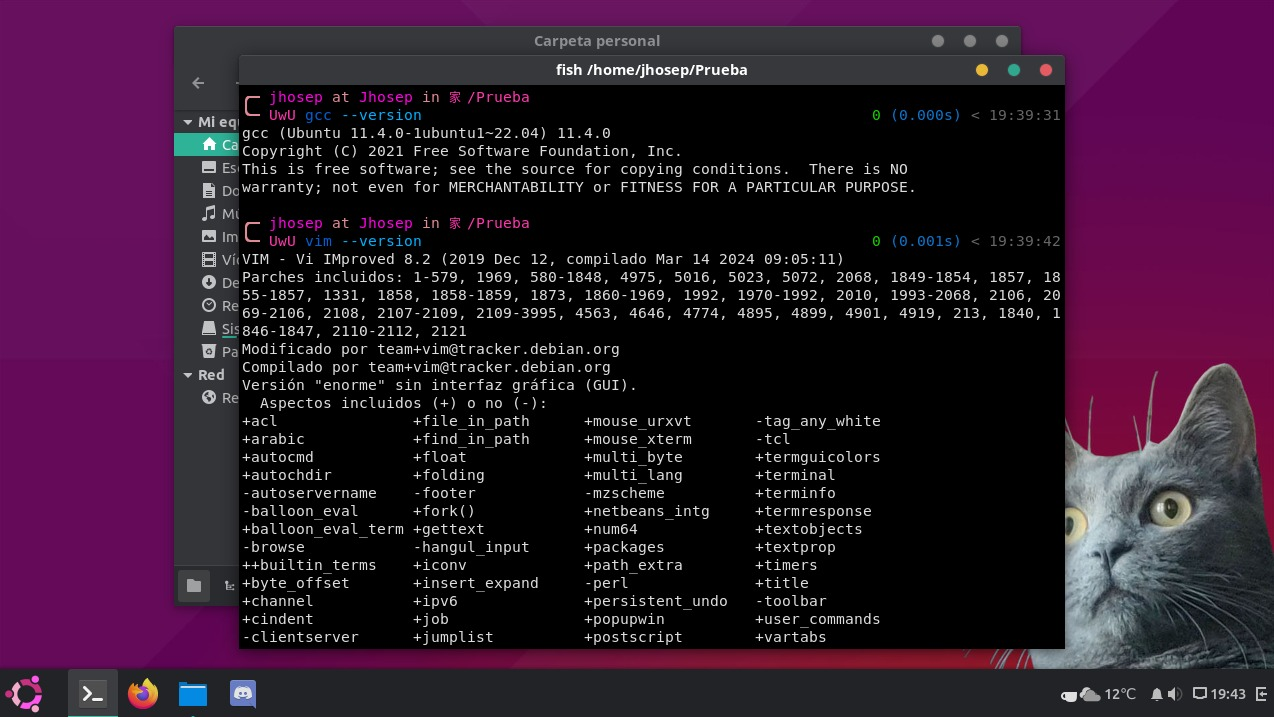
\includegraphics[scale=0.35]{Uwuntu/Versiones1.png}
    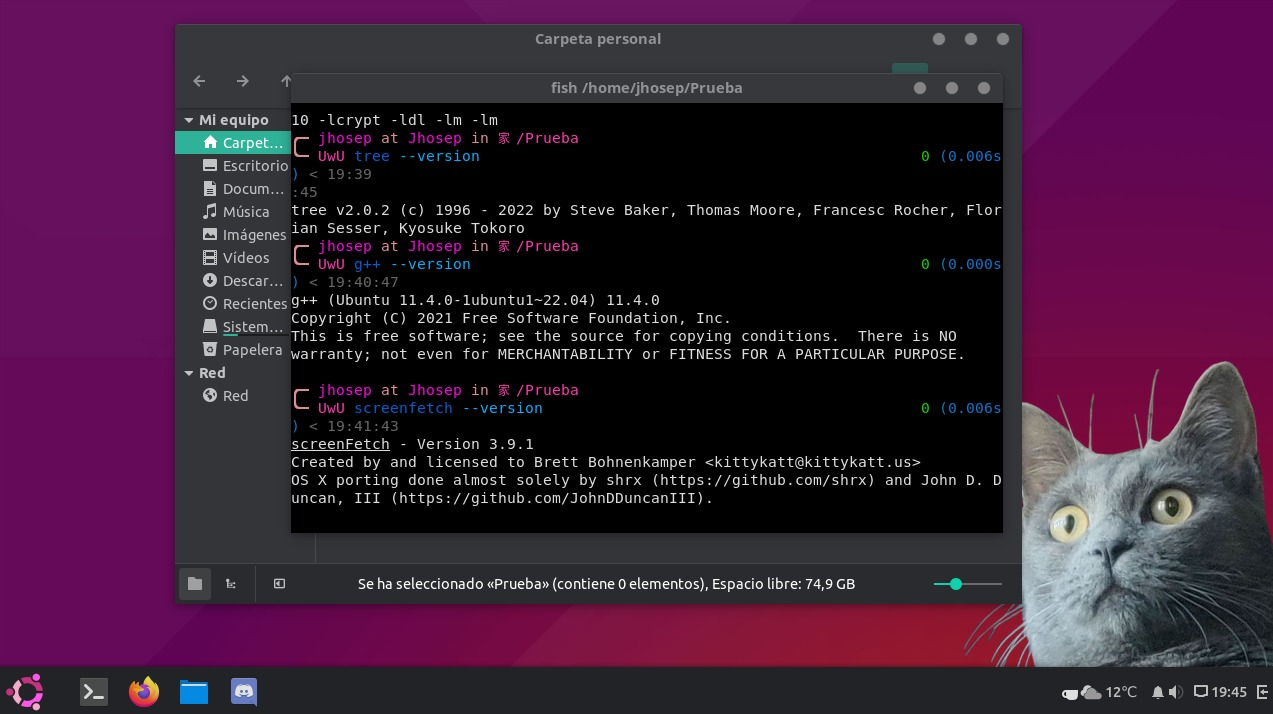
\includegraphics[scale=0.35]{Uwuntu/Versiones2.png}
Ademas se muestran los resultados de los comandos:
\\
    \begin{minted}[tabsize=2,breaklines]{bash}
        UwU uname -a
        UwU screenfetch
    \end{minted}
    
    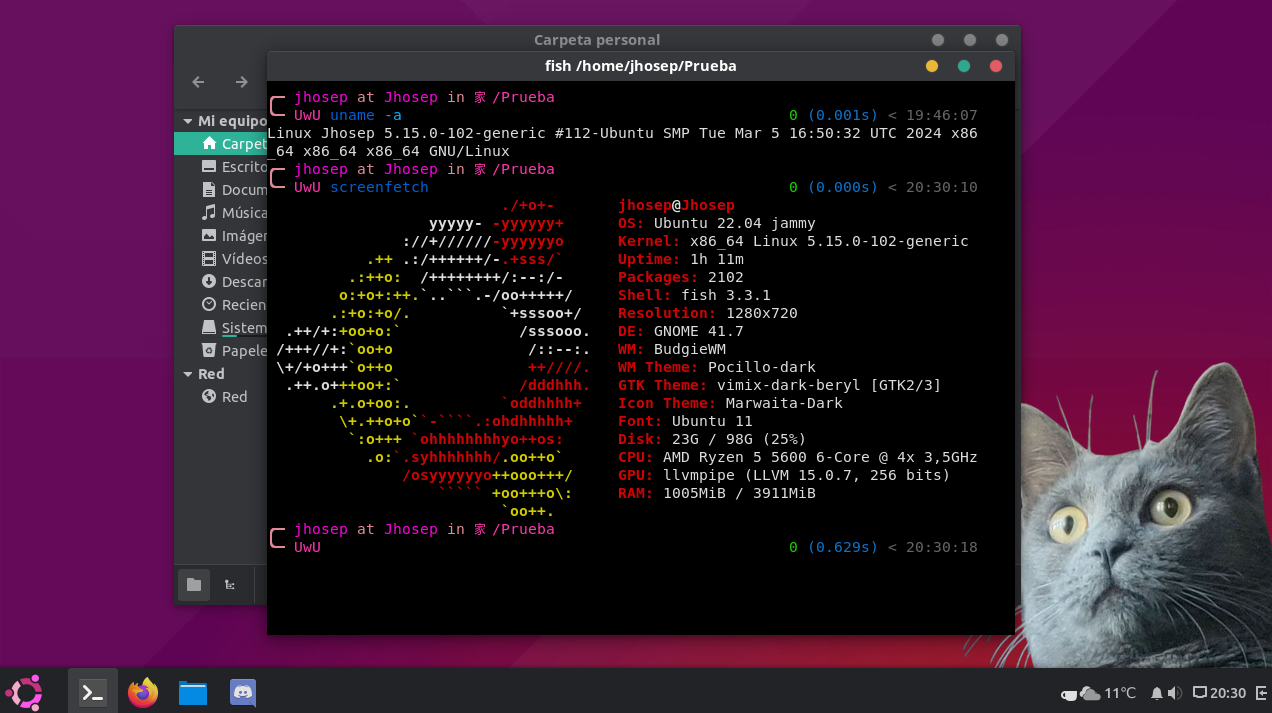
\includegraphics[scale=0.45]{Uwuntu/Comandos.png}
    \newpage
\section{Compilacion C++}

   \subsection{Compilacion Manjaro}
Se crea el directorio, se crea el archivo en \$Home y luego se mueve este al directorio so.
    \begin{minted}[tabsize=2,breaklines]{bash}
        $ mkdir $HOME/so
        $ vi hello.cpp
        $ mv hello.cpp /so/hello.cpp
        $ tree
    \end{minted}
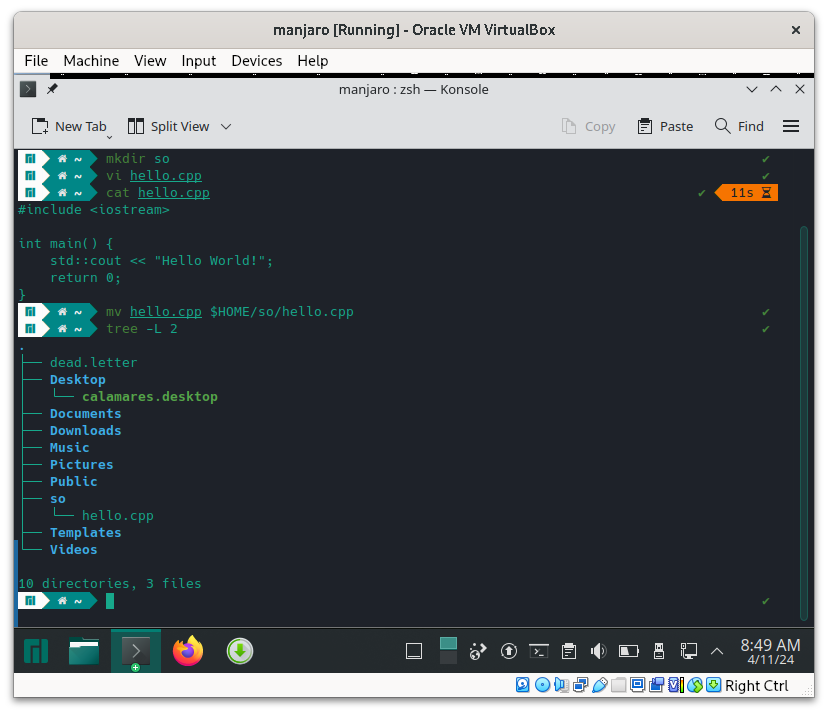
\includegraphics[scale=0.5]{ejer/c++file.png}
\\
\newpage
Para ejecutar el programa primero se compila y luego se ejecuta de la siguiente forma:
    \begin{minted}[tabsize=2,breaklines]{bash}
        $ g++ -o output hello.cpp
        $ ./output
    \end{minted}
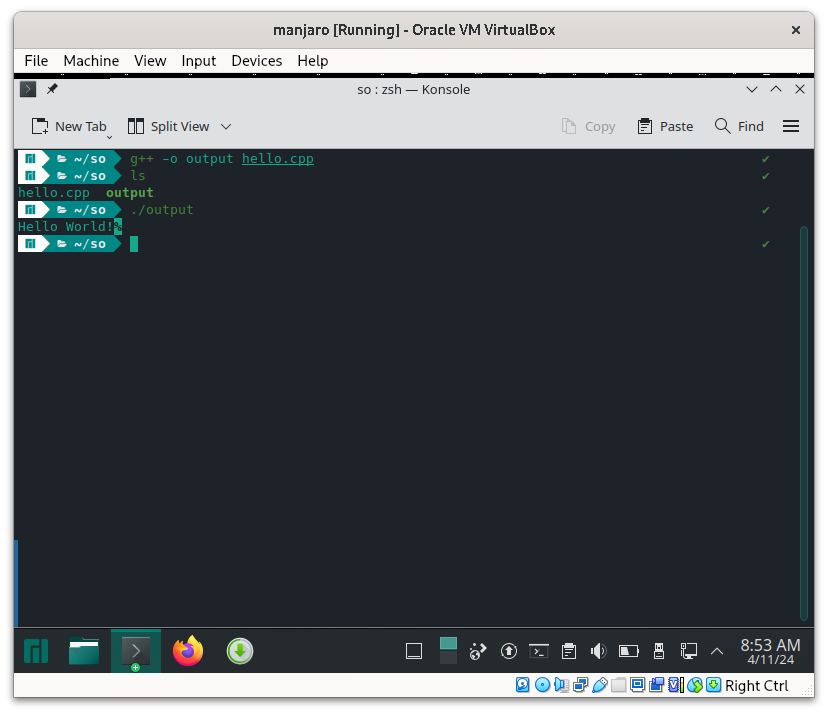
\includegraphics[scale=0.5]{ejer/compilar.png}

\newpage

   \subsection{Compilación UwUntu}
Creamos el directorio en \$Home y creamos el archivo hello.c
    \begin{minted}[tabsize=2,breaklines]{bash}
        UwU $HOME
        UwU mkdir SO
        UwU cd SO
        UwU vim hello.c
    \end{minted}
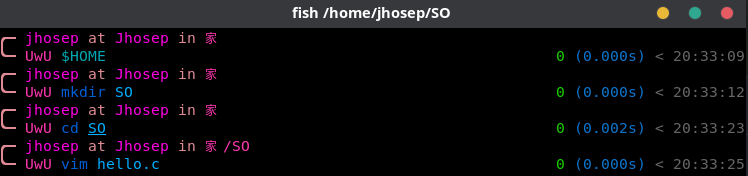
\includegraphics[scale=0.6]{Uwuntu/CreacionHelloc.png}
\\
    \begin{minted}[tabsize=2,breaklines]{bash}
    #include <stdio.h>

    int main() {
        printf("Hola Mundo\n");
        return 0;
    }
    \end{minted}
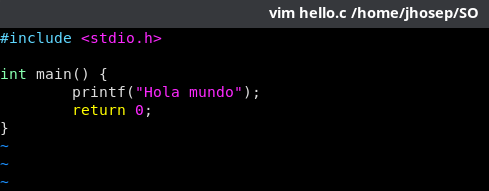
\includegraphics[scale=1.2]{Uwuntu/Holamundo.png}
\\
Y luego compilamos el programa y lo ejecutamos:
    \begin{minted}[tabsize=2,breaklines]{bash}
        UwU gcc hello.c -o hello
        UwU ./hello
    \end{minted}
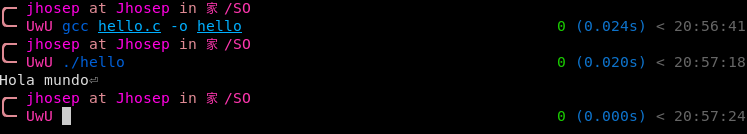
\includegraphics[scale=0.6]{Uwuntu/Ejecucionhelloc.png}
\\

\section{Conclusiones}

\section{Recomendaciones}
\begin{itemize}
    \item No escoger Manjaro para una instalacion minima puesto que al ser una version modificada de Arch su valor agregado esta en la GUI, sin ella sería mejor instalar Arch directamente. Adémas la version minima solo esta disponible para arquitecturas ARM que son bastante dificiles de virtualizar.
    \item 
\end{itemize}



\end{document}